%\documentclass[journal]{IEEEtran}
\documentclass[]{article}

% \renewcommand\IEEEkeywordsname{Keywords}

\usepackage{graphicx}
\usepackage{rotating}
\usepackage{adjustbox}
\usepackage{blindtext}
\graphicspath{ {images/} }
\usepackage{tabularx}
\usepackage{caption}
\usepackage{pdfpages}
\usepackage{amsmath}
\usepackage{float}
\usepackage{xcolor,bytefield}
\usepackage{color,soul}
\pagenumbering{arabic}
\usepackage[margin=1in]{geometry}
\bibliographystyle{IEEEtran}


\providecommand{\keywords}[1]{\textbf{\textit{Keywords:}} #1}
\newcommand{\colorbitbox}[3]{%
	\sbox0{\bitbox{#2}{#3}}%
	\makebox[0pt][l]{\textcolor{#1}{\rule[-\dp0]{\wd0}{\ht0}}}%
	\bitbox{#2}{#3}%
}

\begin{document}
	\markboth{COMPSYS701 - Advanced Digital Systems Design}{}
	
	\begin{titlepage}
		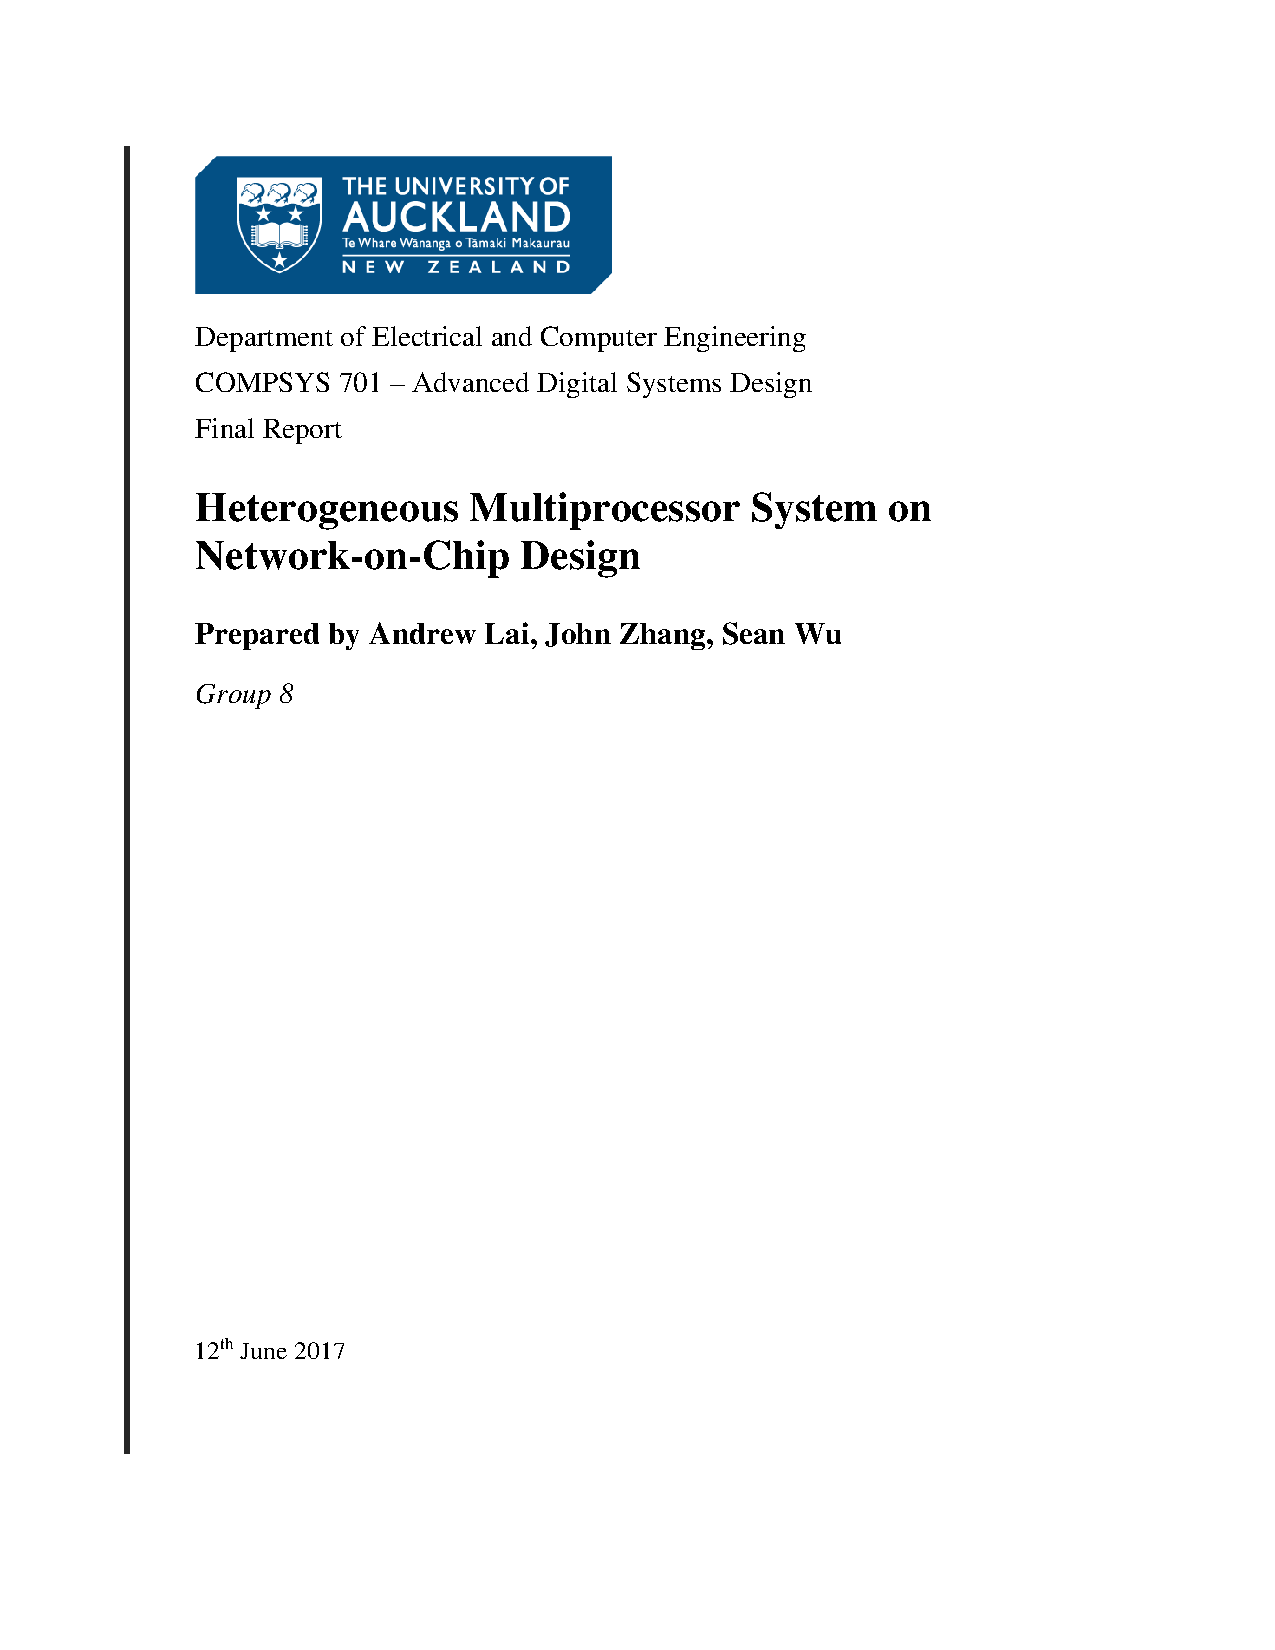
\includepdf[pages={1}]{title_page.pdf}
	\end{titlepage}
	
	\setcounter{page}{2}
	
	\title{\huge \textbf{Heterogeneous Multiprocessor System on Network-on-Chip Design}}
	\author{Group 8 (AJS) - Andrew Lai \texttt{(klai054)}, John Zhang \texttt{(szha215)}, Shiyang Wu \texttt{(swu145)} \\Department of Electrical and Computer Engineering, University of Auckland, New Zealand}
	
	\maketitle
	
	\begin{abstract}
		With Moore’s Law becoming harder to prove, multi-core or multiprocessor systems are becoming more popular ways to improve performance rather than focusing on architecture size or maximum frequency. This report presents a multiprocessor system design based on the Network-on-Chip implemented in System-on-Chip, including designing a new hardware acceleration processor, network interfaces and integrating them alongside existing components using the SystemJ programming language which can run Java programmes on hardware-accelerated Jave Optimised Processors (JOP).
	\end{abstract}
	
	% 	\begin{IEEEkeywords}
	% 		Processor design; Network-on-chip 
	% 	\end{IEEEkeywords}
	
	\keywords{Processor design, Network-on-chip}
	
	\section{Introduction}
	
	%	\begin{figure}[h!]
	%		\centering
	%		\includegraphics[trim={0cm, 0cm, 0cm, 0cm}, clip, width = 3.4in]{pedal_detection_fsm}
	%		\caption{Pedal Detection FSM.}
	%		\label{tumor_L8}
	%	\end{figure}
	
	
	\section{Network-on-Chip Structure}
	
	\subsection{Basic Architecture}
	\begin{figure}[h!]
		\centering
		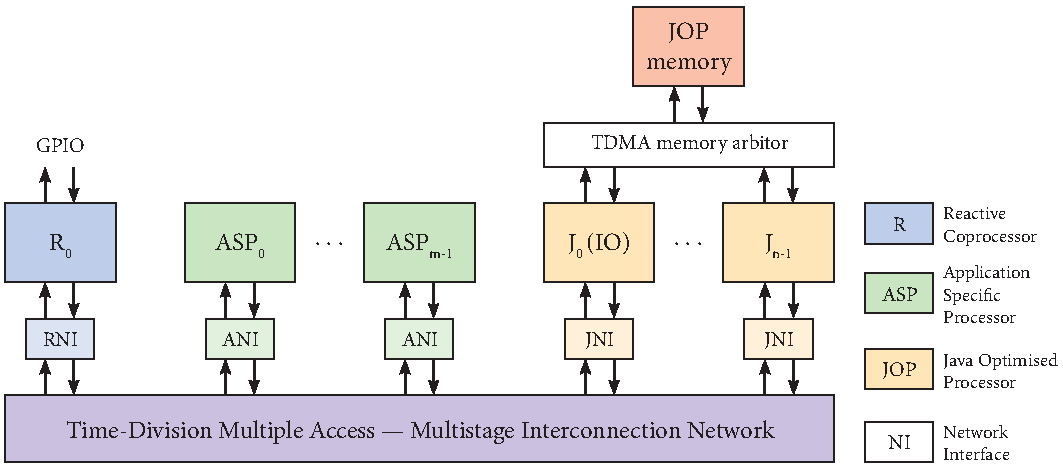
\includegraphics[width = 5.5in]{noc_block_diagram}
		\caption{Top-level diagram of TDMA-MINoC}
		\label{fig:asp_data_path}
	\end{figure}
	
	\subsection{Configuration}
	
	\section{Reactive Coprocessor (AJS)}
	
	\subsection{Control Unit}
	
	\subsection{Datapath}
	
	\subsection{Data Format}
	
	\begin{figure}[H]
		\centering
		\captionsetup{justification=centering,margin=2cm}
		\begin{bytefield}[endianness=big,boxformatting={\centering},
			bitwidth=1em,bitheight=8mm]{32}
			\bitheader{0-31} \\
			\bitbox{1}{\rotatebox{90}{\tiny valid}}
			\bitbox{1}{\rotatebox{90}{\scalebox{.5}{Legacy(0)}}} &
			\colorbitbox{lightgray}{2}{\tiny Unused} & 
			\bitbox{4}{\small JOP ID} &
			\bitbox{8}{\small Clock-domain ID} & 	
			\bitbox{16}{Address to Java Method} & 
		\end{bytefield}
		\caption{ReCOP\_AJS Data-call Packet}
		
	\end{figure}
	
	
	\begin{figure}[H]
		\centering
		\captionsetup{justification=centering,margin=2cm}
		\begin{bytefield}[endianness=big,boxformatting={\centering},
			bitwidth=1em,bitheight=8mm]{32}
			\bitheader{0-31} \\
			\bitbox{1}{\rotatebox{90}{\tiny valid}}
			\bitbox{1}{\rotatebox{90}{\scalebox{.5}{Legacy(0)}}} &
			\bitbox{6}{\small ReCOP ID} & 
			\bitbox{12}{\small Writeback Address} &
			\colorbitbox{lightgray}{10}{\small Unused} & 	
			\bitbox{1}{\rotatebox{90}{\tiny IRQ(1)}} &
			\bitbox{1}{\rotatebox{90}{\tiny Result}}
		\end{bytefield}
		\caption{ReCOP\_AJS Data-call Result Packet}
		
	\end{figure}
	\subsection{Simulation}
	
	
	\section{Application Specific Processor}
	
	\subsection{Control Unit}
	
	\newpage
	\subsection{Datapath}
	% 		\begin{turn}{-90}
	% 		\begin{minipage}{0in}
	%     		\centering
	%     		\hspace*{-0.7in}
	%     		\vspace*{-0.5in}
	%     		    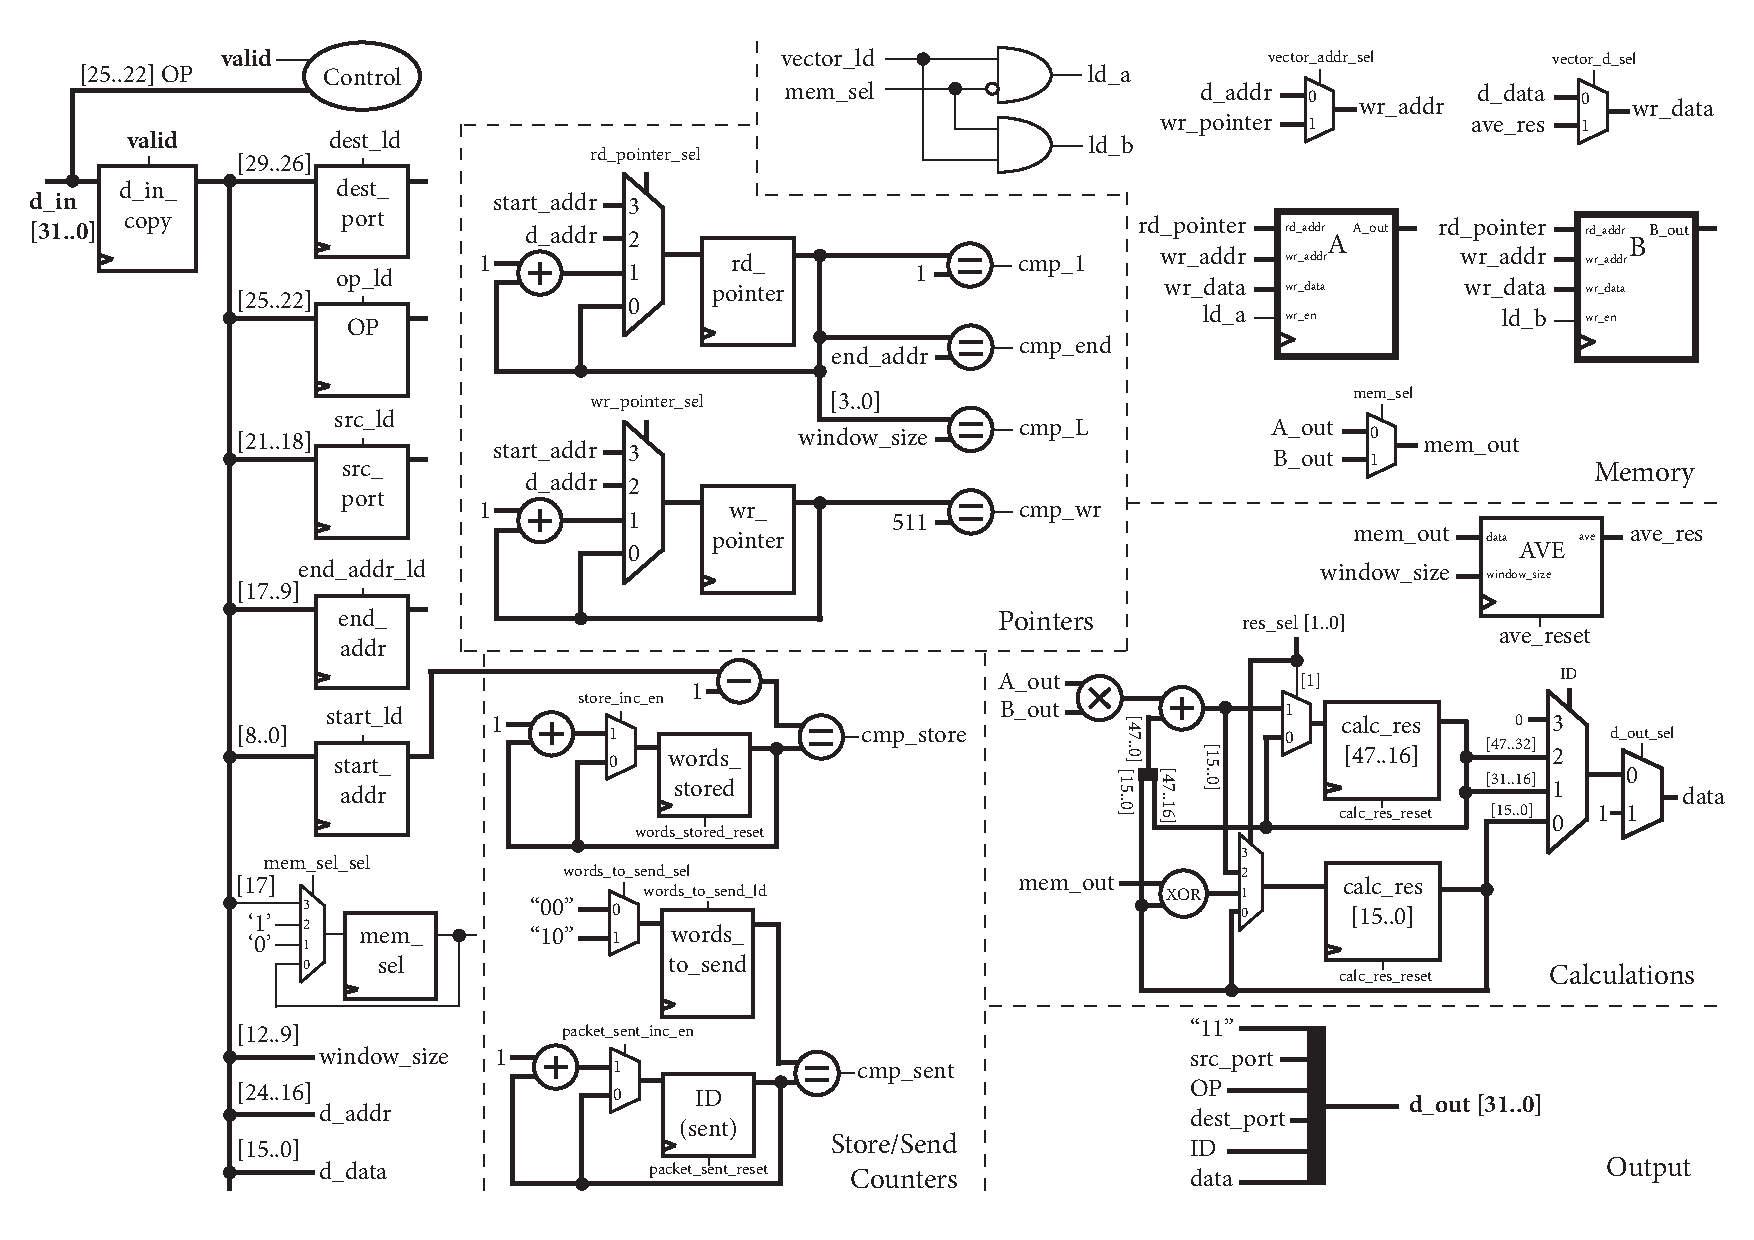
\includegraphics[width = 8.9in]{asp_datapath_v3}
	%     		    \caption{ASP datapath}
	%     		    \label{fig:asp_datapath}
	% 	    \end{minipage}
	% 	    \end{turn}
	
	
	% \begin{sidewaysfigure}
	% 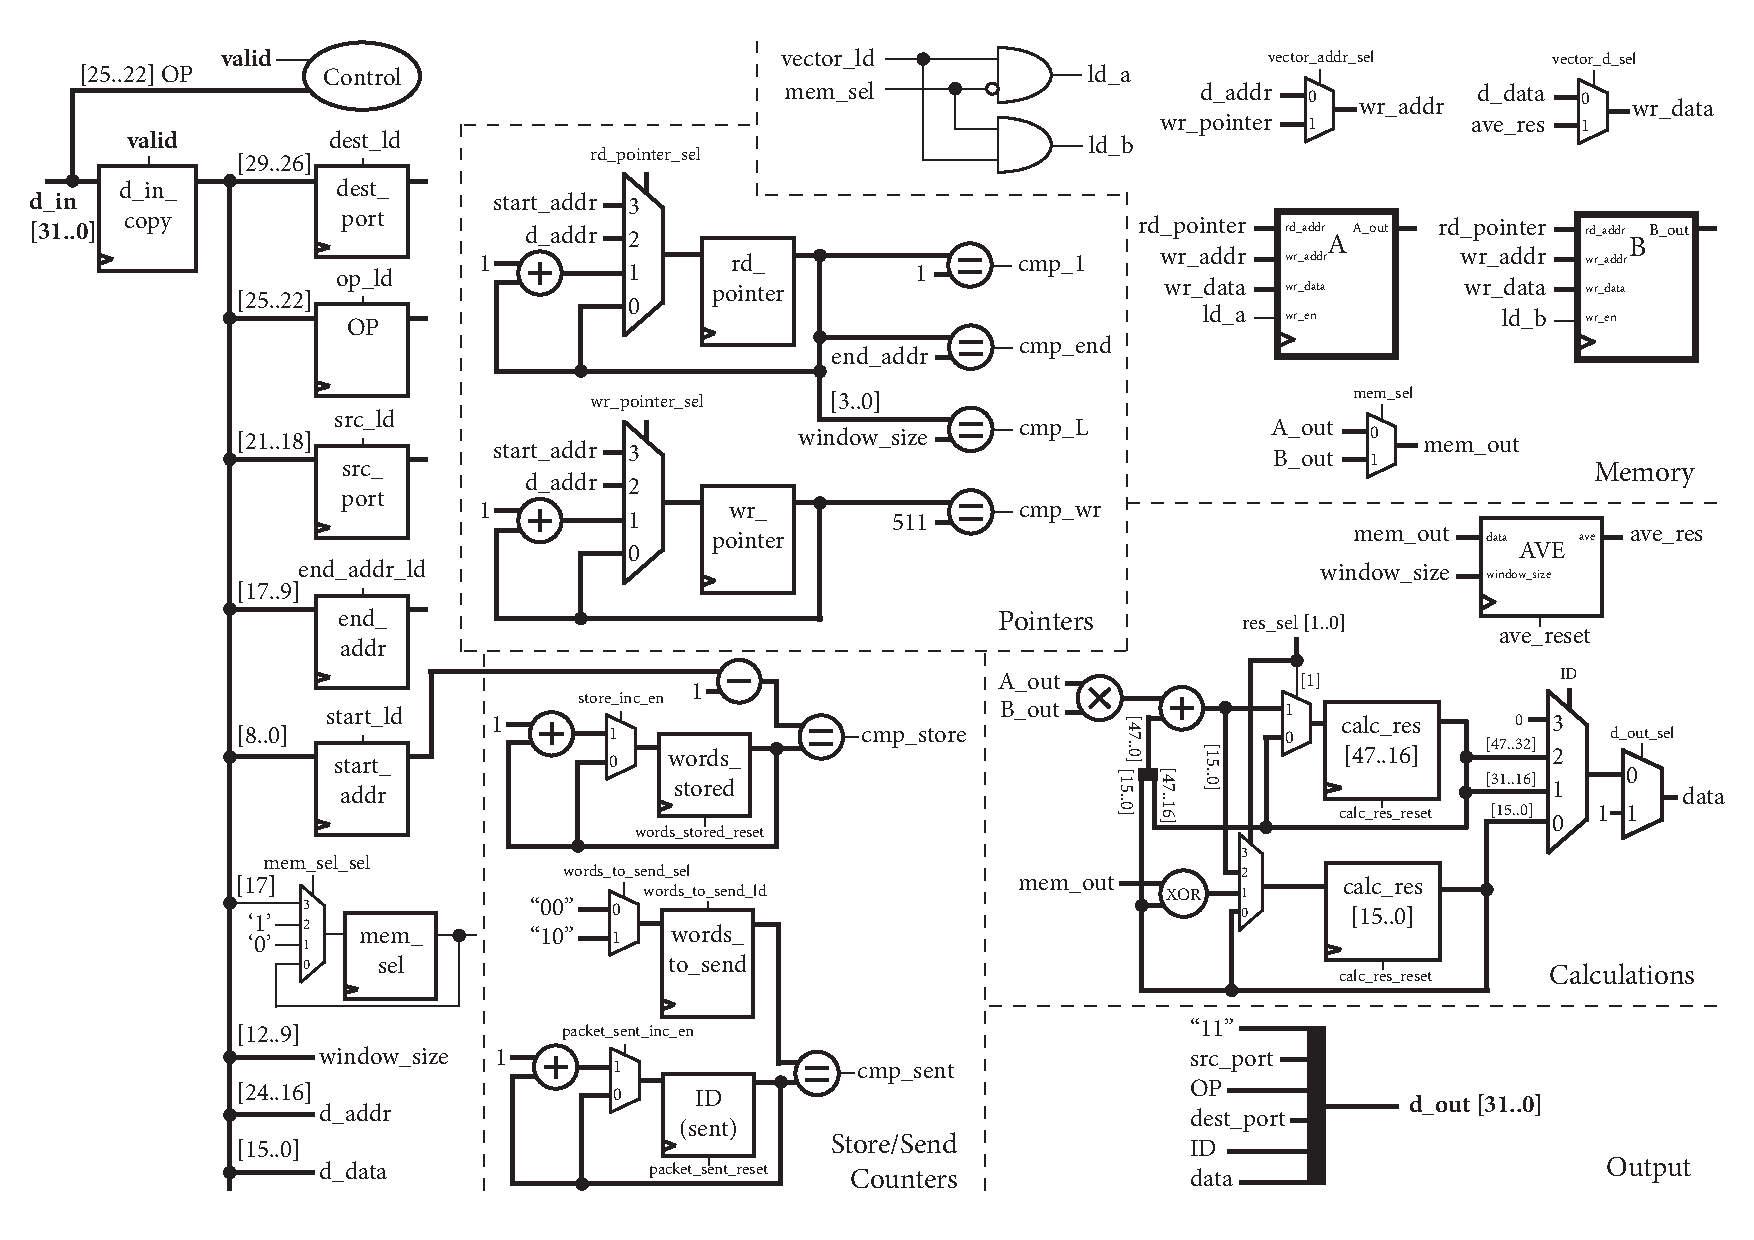
\includegraphics[width=8.9in]{asp_datapath_v3}
	% \caption{ASP datapath}
	% \label{fig:fig1}
	% \end{sidewaysfigure}
	
	\begin{figure}[H]
		\begin{adjustbox}{addcode={\begin{minipage}{\width}}{\caption{%
				ASP datapath.
				}\label{fig:asp_datapath}\end{minipage}},rotate=-90,center}
			\hspace*{-0.7in}
			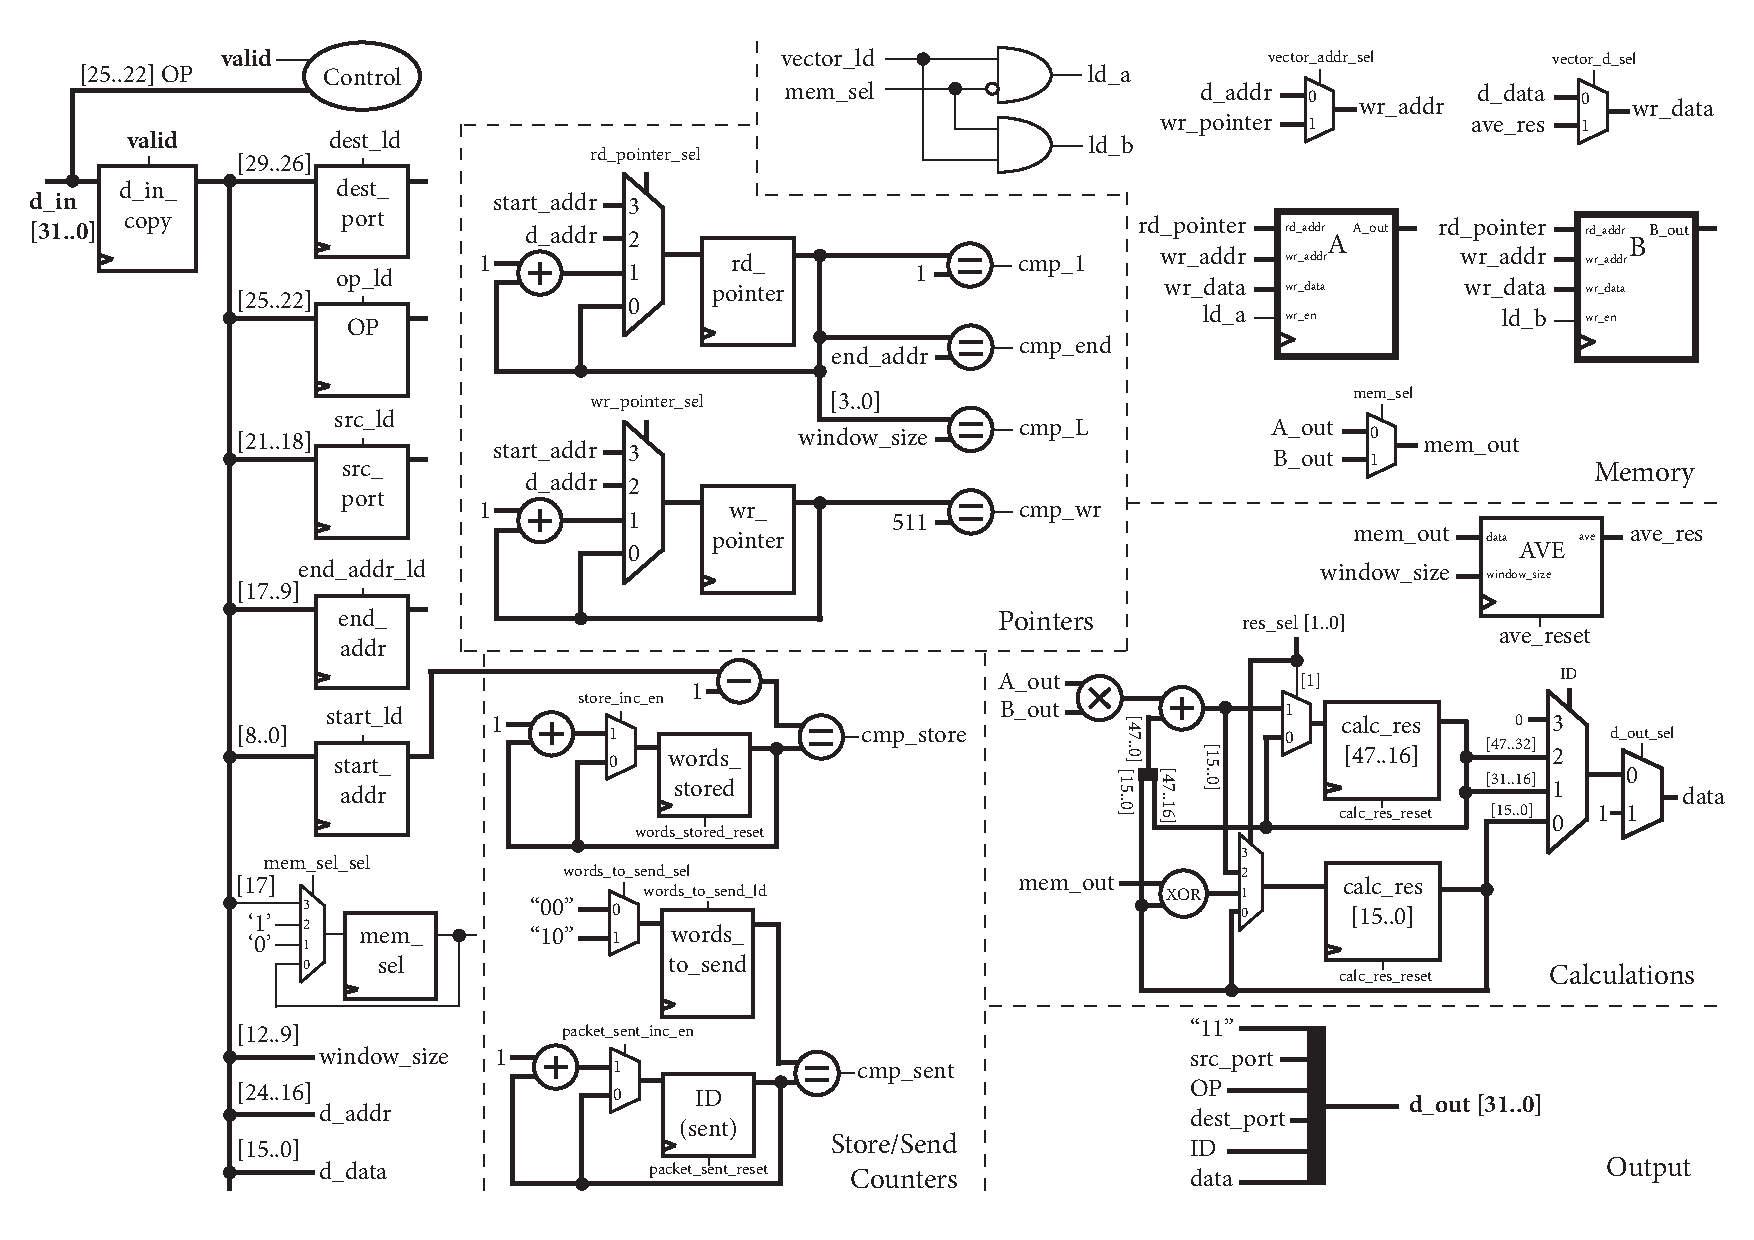
\includegraphics[scale=.8]{asp_datapath_v3}%
			
		\end{adjustbox}
	\end{figure}
	
	Fig. \ref{fig:asp_datapath} shows the datapath of the ASP.
	
	\begin{figure}[h!]
		\centering
		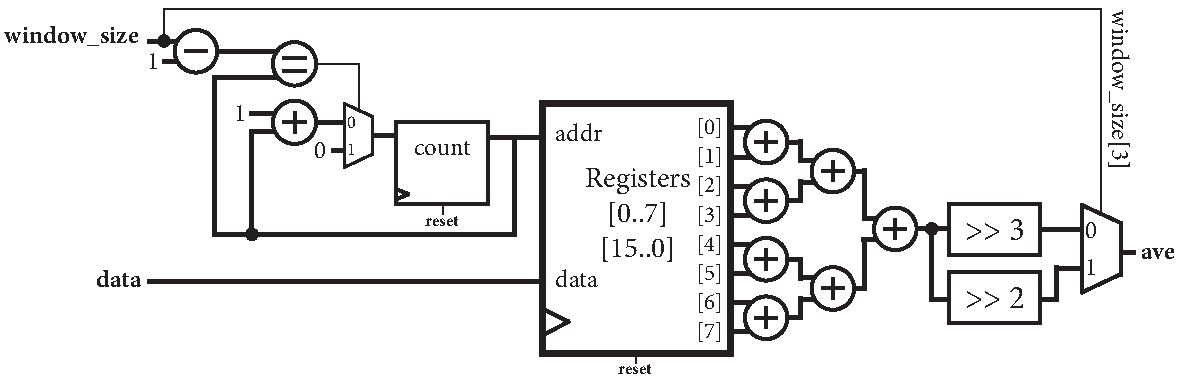
\includegraphics[width = 5.5in]{ave_filter_datapath}
		\caption{Average Filter datapath}
		\label{fig:ave_filter_datapath}
	\end{figure}

	\subsection{Operations}
	\subsubsection{Store Reset}
	Resets either vector A or vector B to 0 depending to the \texttt{mem\_sel} bit. Returns \texttt{Operation Complete} (formerly known as \texttt{Access Granted} packet -- 0x0001). 
	
	\subsubsection{Store}
	This operation will store a fixed number of words to the ASP internal memory. It will send two types of packets -- a Store Invoke packet, followed by a series of Data packets (see section \ref{sec:asp_data_format}). The Store Invoke packet contains information on the number of words and which vector to be stored in. Data packets contains the 16-bit data and 9-bit address indicating the memory location to be stored at. The number of data packets must match the store invoke packet's specified number of words. An 
	\subsubsection{XOR}
	This function will perform a bit-wise XOR operation to the specified vector from index \texttt{begin address} to \texttt{end address} inclusively. After the operation, ASP will send the result to the ANI.
	\subsubsection{MAC}
	Multiply and Accumulate will perform a dot product opertion between index \texttt{m} to \texttt{n} for vector A and B. 
	\begin{equation}
	S = \sum_{i=m}^{n}A(i)B(i)
	\end{equation}
	There is a high probability that the MAC result will overflow a 16-bit data structure, with possible maximum being 41 bits.
	\begin{equation}
	(2^{16})^2 \times 512 = 2^{41}
	\end{equation}
	
	\par
	41-bit data can be sent as 3 packets of 16 bits. To stay consistent, the ASP will always send 3 packets consecutively. In order to differentiate between the packets, a 2-bit packet ID is inserted into each packet, from 0 to 2. ID 0 being the first packet and ID 3 being the last. It is up to the JOP programme to concatenate those 3 packets into a \texttt{long}.
	
	\subsubsection{AVE}
	Average filters vector A or B with a run-time window size (L) of 4 or 8 using the algorithm described in (\ref{eq:ave}). The datapath of the AVE block in Fig. \ref{fig:ave_filter_datapath} shows that the 8 internal registers are always summed and right shifted by 2 or 3 depending on the window size, and data is always stored at data registers at index \texttt{count}. The \texttt{count} is an up counter that resets after its value is \texttt{window size} - 1, as the register indexing is 0 to 7, while the \texttt{window size} can be 4 or 8. \\
	
	\begin{equation} \label{eq:ave}
	X(i) = \sum_{k = i}^{i+L-1} \frac{X(k)}{L} \quad \text{where} \; i \in [0,N-L)
	\end{equation}	
	
	This allows pipelining, since it is always averaging a stream of data coming in, replacing the oldest. Upon initialisation, the registers are reset, \texttt{rd\_pointer} points at 0 and starts to increment by 1, \texttt{wr\_pointer} is set to point at 0, but not incrementing. When \texttt{rd\_pointer} is equal to the \texttt{window size}, the \texttt{AVE} registers will be filled, outputting the first average value, and \texttt{cmp\_L} will be high. The \texttt{cmp\_L} signal triggers a state transition, and \texttt{wr\_pointer} starts incrementing, and \texttt{vector\_ld} is set high in order to write into memory. This continues until the \texttt{rd\_pointer} overflows and equal to 1 -- when the element 

	\subsection{Data Format}\label{sec:asp_data_format}
	
	\begin{figure}[H]
		\centering
		\captionsetup{justification=centering,margin=2cm}
		\begin{bytefield}[endianness=big,boxformatting={\centering},
			bitwidth=1em,bitheight=8mm]{32}
			\bitheader{0-31} \\
			\bitbox{1}{\rotatebox{90}{\tiny Valid}}
			\bitbox{1}{\rotatebox{90}{\scalebox{.5}{Legacy(1)}}} &
			\bitbox{4}{\small Dest} & 
			\bitbox{4}{\small OP code} &
			\bitbox{4}{\small Source} & 	
			\bitbox{1}{\rotatebox{90}{\tiny Mem sel}} &
			\colorbitbox{gray}{8}{\small Unused} &
			\bitbox{9}{\small Number of words} & 
		\end{bytefield}
		\caption{Store invoke packet format to ASP}
		
	\end{figure}
	
	
	\begin{figure}[H]
		\centering
		\captionsetup{justification=centering,margin=2cm}
		\begin{bytefield}[endianness=big,boxformatting={\centering},
			bitwidth=1em,bitheight=8mm]{32}
			\bitheader{0-31} \\
			\bitbox{1}{\rotatebox{90}{\tiny Valid}}
			\bitbox{1}{\rotatebox{90}{\scalebox{.5}{Legacy(1)}}} &
			\bitbox{4}{\small Dest} & 
			\colorbitbox{gray}{1}{\rotatebox{90}{\tiny Unused}} &
			\bitbox{9}{Address} & 	
			\bitbox{16}{Data} &
			
		\end{bytefield}
		\caption{Data packet format to ASP}
		
	\end{figure}
	
	
	\begin{figure}[H]
		\centering
		\captionsetup{justification=centering,margin=2cm}
		\begin{bytefield}[endianness=big,boxformatting={\centering},
			bitwidth=1em,bitheight=8mm]{32}
			\bitheader{0-31} \\
			\bitbox{1}{\rotatebox{90}{\tiny Valid}}
			\bitbox{1}{\rotatebox{90}{\scalebox{.5}{Legacy(1)}}} &
			\bitbox{4}{\small Dest} & 
			\bitbox{4}{\small OP code} &
			\bitbox{4}{\small Source} & 	
			\bitbox{9}{\small End Address (inc)} &
			\bitbox{9}{\small Begin Address (inc)} & 
		\end{bytefield}
		\caption{Command invoke packet format to ASP}
		
	\end{figure}
	
	\begin{figure}[H]
		\centering
		\captionsetup{justification=centering,margin=2cm}
		\begin{bytefield}[endianness=big,boxformatting={\centering},
			bitwidth=1em,bitheight=8mm]{32}
			\bitheader{0-31} \\
			\bitbox{1}{\rotatebox{90}{\tiny Valid}}
			\bitbox{1}{\rotatebox{90}{\scalebox{.5}{Legacy(1)}}} &
			\bitbox{4}{\small Dest} & 
			\bitbox{4}{\small OP code} &
			\bitbox{4}{\small Source} & 	
			\colorbitbox{yellow}{2}{\small \hl{\textbf{ID}}} &
			\bitbox{16}{\texttt{Data} or \texttt{OperationComplete}} & 
		\end{bytefield}
		\caption{Result packet format from ASP}
		
	\end{figure}
	
	The \texttt{last bit} in the original design was not used.
	
	\section{ASP Network Interface}
	In order for the ASP to communicate with the rest of the system, a network interface, ANI has been designed. The ANI contains two Altera Megafunction First-in-first-out (FIFO) queues to ensure all packets are sent and received. 
	\subsection{Datapath}
	
	\begin{figure}[H]
		\centering
		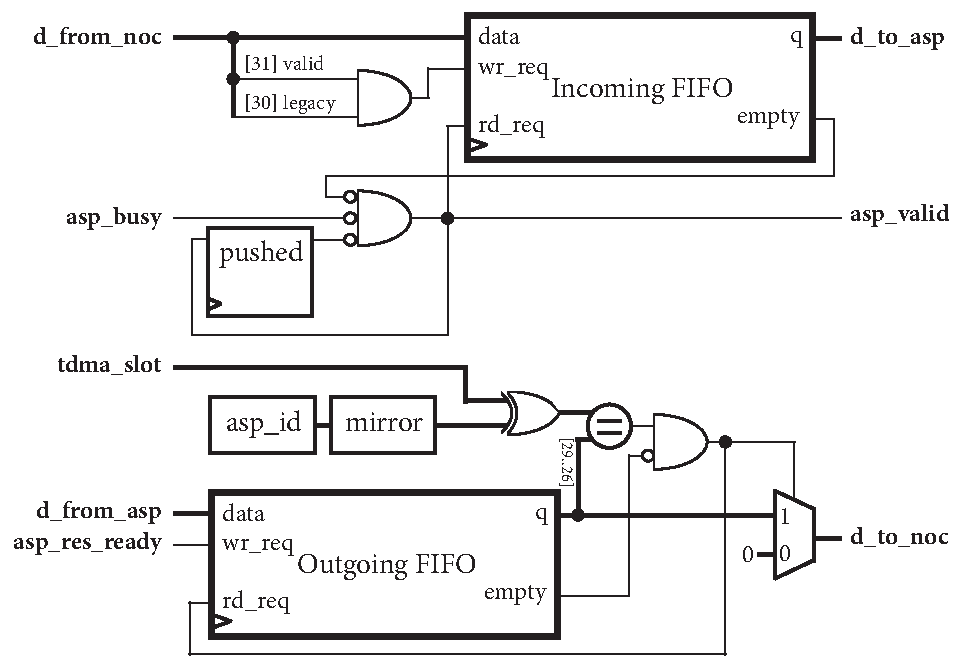
\includegraphics[width = 5in]{ani_datapath}
		\caption{ANI datapath}
		\label{fig:ani_datapath}
	\end{figure}
	
	\subsection{Interaction with TDMA-MIN}
	
	\subsection{Timing}
	
	\subsection{Simulation}
	
	\subsection{Sythesis}
	
	\subsection{FPGA Testing}
	
	\subsection{Performance Analysis}
	
	
	
	\section{JOP Network Interface}
	
	
	
	\section{Java Programmes}
	
	\subsection{ASP APIs}
	Serveral APIs are provided in the \texttt{ASPCommunication} class. The developer has the responsibility of calling them using the correct \texttt{ASPid}, which specifies the ASP this packet is intended for. JNI will handle the correct ports, for the particular ASP ID. The number of ASPs is specificed in the top-level configuration file. The list of APIs implemented is:
	\begin{enumerate}
		\item \texttt{private static void sendPacket(int packet);}\par
		Writes the packet to the data call result register, which will be sent to the JNI and out to the NoC. Used by the other public methods.\\ \par
		
		\item \texttt{public static int pollASPResponse();}\par
		Polls the datacall register, checks \emph{valid} bit.\\ \par
		
		\item \texttt{public static int storeReset(int ASPid, int memSel);}\par
		Sends the reset instruction to ASP with \texttt{ASPid} and reset its vector depending on the value of \texttt{memSel}.\\ \par
		
		\item \texttt{public static int store(int ASPid, int[] data, int start, int memSel);}\par
		Sends a store instruction to ASP of \texttt{ASPid} with an Integer array. The instruction will command ASP to store the array from \texttt{start} to \texttt{data.length} to vector specified by \texttt{memSel}.\\ \par
		
		\item \texttt{public static int xor(int ASPid, int memSel, int start, int end);}\par
		Sends an xor instruction to ASP with \texttt{ASPid}. The addresses of xor instruction is from \texttt{start} to \texttt{end}.\\ \par
		
		\item \texttt{public static long mac(int ASPid, int start, int end);}\par
		Sends a mac instruction to ASP with \texttt{ASPid}. The addresses of mac instruction is from \texttt{start} to \texttt{end}. ASP will return 3 packets of data and this API will return the cacatenated data with a long type.\\ \par
		
		\item \texttt{public static int ave(int ASPid, int windowSize, int memSel);}\par
		Sends an ave command to ASP with \texttt{ASPid}. \texttt{windowSize} specifies the window size of the moving average filter.\\ \par
		
	\end{enumerate}
	
	All of the above listed APIs are blocking - the programme will freeze until the ASP has responded with the expected number of packets. However, this can cause time predictability issues and greatly increase the tick duration, which is undesirable. A potential solution has been provided in Section \ref{sec:future_work}.
	
	
	
	
	\subsection{Multi-JOP Programme}
	
	A simple multi-JOP Java program was developed to perform a simple matrix multiplication:
	\begin{equation}
	\textbf{C} = \textbf{A} \times \textbf{B}
	\end{equation}
	\begin{equation}
	\textbf{A} = \begin{pmatrix}	2&3&5&2&3\\	3&2&3&4&1 \\ 2&3&1&2&3	\end{pmatrix}
	\quad
	\textbf{B} = \begin{pmatrix} 1&2 \\ 2&3 \\ 6&5 \\ 1&2 \\ 2&2 \end{pmatrix}
	\quad
	\textbf{C} = \begin{pmatrix} 46&48 \\ 31&37 \\22&28 \end{pmatrix}
	\end{equation}
	
	For the purpose of multi-JOP computation, each JOP will perform a row of matrix multiplication. Therefore for $JOP_i, i \in [0,2]$, the calculations it will perform are:
	\begin{equation}
	\sum\limits_{j=0}^{L}\textbf{C}_{ij} = \sum\limits_{k=0}^{N} \textbf{A}_{ki} \times \textbf{B}_{jk}
	\end{equation}
	Where $L$ is the number of columns of $\textbf{C}$, and $N$ is the number of columns of $\textbf{A}$. Notice the number of rows of $\textbf{B}$ is equal to $N$ as well.
	\section{Integration}
	
	\subsubsection{SystemJ Program}
	
	
	
	\section{Future Work} \label{sec:future_work}
	Due to time constraints in the project, several parts of the design can be further improved.
	
	\subsection{ReCOP}
	Pipeline Ready TM
	
	\subsection{ASP}
	
	
	\subsection{ANI}
	
	
	\subsection{Java API}
	As mentioned in section JAVA APIS, the APIs are blocking. A possible fix is to create an object of the ASPCommunication class, storing the the current progress of the datacall. For storing data, the complete array can be divided into smaller arrays by keeping track of the indices and only send one smaller block per tick. While waiting for a response, instead of blocking poll, create a separate method responsible for polling and checking the OP code in the response packet
	
	
	
	\section{Conclusion}
	
	
	
	\section{Acknowledgements}
	The authors would like to thank Professor Zoran Salcic and Dr Morteza Biglari-Abhari for their lectures on RTL, processor, and system designs, (soon-to-be Dr) Benjamin Tan, (soon-to-be Dr) Nicholas Harvey for their continuous guidance and support on this project. The authors would also like to thank Dr Heejong Park for his guidance and support for existing portions of the project.
	
	
	\section{References}
	
	
	
	\section*{Appendix}
	
	
	
\end{document}

